\chapter{Numerical Solvers in Physics Based Simulation} \label{Chapter:Solver}
In the pipeline of physics based simulation, the complexity of majority of the stages are simply $O(N)$, where $N$ is the number of unknowns, while the complexity of the solve stage can be as much as $O(N^2)$. For high resolution simulation, the solve stage can often take over 90\% of the simulation time. There are two major categories of numerical solvers, direct solvers and iterative solvers. 

Direct solvers provide solution at the precision of the numerical limit, and they generally operates in sparse matrix format (for instance Compressed Sparse Column). Therefore they can be used in arbitrary discretization and problems, but they have the minimal cost of $O(N^2)$ and memory footprint of $O(N^{\frac{4}{3}})$ or higher. This super-linear cost makes direct solvers infeasible for high resolution simulations. But for small scale simulations, direct solver algorithms such as Cholesky factorization are attractive for their accuracy and robustness. 

Iterative solvers, on the other hand, as the name suggests, provides a solution that converges to the exact solution with each iteration. Some iterative solvers, such as Conjugate Gradient Method[\cite{nocedal2006conjugate}] and Generalized Minimal Residual algorithm\cite{saad1986gmres}], mathematically speaking, can achieve the exact solution at the $N$th iteration. At the cost of $O(N)$ per iteration, it will give the exact solution with $O(N^2)$ cost. But in practice, due to numerical drift, those algorithm will require restarts for large problems, and can't achieve the exact solution to numerical limit. 

For large problems, an iterative solver is preferred over direct solver for two major reasons: 1. the memory footprint of an iterative solver is usually $O(N)$, which allows larger problems to fit into memory. 2. Though iterative solve can potentially takes longer to achieve solution at numerical limit, the option to terminate early in exchange for an approximate solution is attractable when computation time is limited. But at higher and higher resolution, iterative solvers can take considerably longer to converge and sometimes even stagnate (See results in Chapter \ref{Chapter:Elasticity}). If terminates too early, the poorly approximated solution can lead to unphysical results, due to that the solution can not satisfies the governing equation.

\section{Multigrid Method}
\subsection{Overview}
Multigrid method was proposed in work [\cite{brandt1977multi}]. The multigrid fundamental idea lies as follows: we start with a set of grids $G^0$,$G^1$,...,$G^M$, which are all discretization of the same domain $\Omega$. With higher level consists of a coarser elements. In our uniform grid discretization, int 1D, if the nodes in $G^0$ lies on points $(0,h,2h,3h,4h...)$. We can construct the next level $G^1$ as nodes on points $(0,2h,4h,6h,8h...)$.

If our continuous PDE of the boundary value problem takes the form:
\begin{equation}
LU(x) = F(x)\text{, in }\Omega,  \Lambda U(x) = \Phi(x)\text{, on the boundary }\partial\Omega
\end{equation}
Here, $L$ and $\Lambda$ are the differential operators that are on the interior of the domain and the boundary respectively. $U(x)$ is the solution we seek. $F(x)$ and $\Phi(x)$ are the loading condition that are given. We can now write the discretized PDE at each level $k$ as:
\begin{equation}\label{equ:mg_operator}
L^kU^k(x) = F^k(x)\text{, for} x \in G^k,  \Lambda^k U^k(x) = \Phi^k(x)\text{, for} x\in\partial G^k 
\end{equation}
Now, $L^k$ and $\Lambda^k$ are linear operators and can be perceived as matrices. We are interested in acquiring the solution at the finest level. The main idea is, if at $k$th level, the solution $U^k(x)$ is a good approximation to the continuous $U(x)$. We can use the $k$th level solution as a potent guess for the $k-1$ level. Then apply a correction routine we call \textbf{smoother} that is $O(|G^{k-1}|)$ cost to bring the guess close to solution. This process is repeated until $U^0(x)$ is considered close enough to the solution. 

Multigrid has the property that each iteration can reduce the error by at least a constant factor $W$. That is $\frac{|\mathbf{e}_{i+1}|}{|\mathbf{e}_{i}|}<W$. Here we take $|\mathbf{e}|$ as the infinite norm of $\mathbf{e}$. What the value of $W$ is depends on the PDE, how the discretization of each level is constructed, and how potent the smoother is. The convergence property of multigrid will  be elaborate more in later section. But we can see that if we seek to reduce the error by 6 orders of magnitude, we will need $-\log_W 10^6$ iterations to converge, which is a constant. For instance if $W = 0.5$, it will take at most 20 iterations to converge. But, of course, in bad cases, for instance, when $W = 0.99$, it will take about 1400 iterations.

Now we have introduced some fundamental multigrid concepts, let's take a deep look at multigrid implementations.
\subsection{Construction of the Hierarchy}
For constructing the discretized hierarchal operators in equations \ref{equ:mg_operator}, there are two common ways, geometric coarsening and Galerkin coarsening. In work [\cite{zhu2010efficient}], [\cite{mcadams2010parallel}], geometric coarsening was used to construct hierarchal operators. For the domain decomposition solver, geometric coarsening based multigrid is also it's building block, but more on that later. 

But in many cases, only the top level operator is provided to the solver, and the underlining PDE is inaccessible, re-discretization of the PDE with a coarser grid(or mesh) is not an option, in those cases, Galerkin coarsening is usually used for constructing the hierarchy, such as in work [\cite{dendy1982black}], [\cite{brezina2001algebraic}], and [\cite{dohrmann2007interpolation}]. This is also our method for the multigrid construction in our SIMD-optimized solver for topology optimization.  

When the underlining PDE is unavailable, there is the possibility to acquire the geometric coarsened operator through homogenization of Galerkin coarsened operator which is demonstrated in work [\cite{moulton1998black}]. But this is aspect is not the focus of this work. Therefore I will leave out here the discussion of homogenization.
\subsection{Geometric Coarsening}
Geometric coarsening refers to the method of constructing the Multigrid hierarchy through re-discretization with different grid size. It has been proven effective for both homogeneous Poisson[\cite{mcadams2010parallel}] and homogeneous elasticity[\cite{zhu2010efficient}]. Here I will take finite difference Poisson discretization as an example to demonstrates the geometric coarsening principles and its limitation. For more details, I would refer the reader to the work[\cite{mcadams2010parallel}].

The continuous PDE of homogeneous Poisson can be written as:
\begin{equation}
\Delta p\mathbf{x} = f\mathbf{x} \text{ in } \Omega \in \mathcal{R}^3
\end{equation}
$$
p(\mathbf{x}) = \alpha(\mathbf{x}) \text{ on } \Gamma_D\text{, } p_n(\mathbf{x}) = \beta(\mathbf{x}) \text{ on } \Gamma_N
$$
The finite difference discretization on a uniform grid of size $h$, samples points we denote as $\{i,j,k\} \in \mathcal{N}^3$ that corresponding to geometric location $\{ih,jh,kh\} \in \Omega$. The finite difference discretized operator for the interior can be written as:
\begin{equation}
\sum_{i',j',k'\in \mathcal{N}_{[i,j,k]}}\frac{p_{[i',j',k']}-p_{[i,j,k]}}{h^2} = f_{[i,j,k]}
\end{equation}
$$
\mathcal{N}_{[i,j,k]} = \{(i\pm1,j,k),(i,j,k\pm1),(i,j,k\pm1)\}
$$
It is a 2nd order accurate discretization as we can write:
$$
\frac{\partial^2 p}{\partial x^2}(x_0) = \frac{p(x_0)-p(x_0)}{h^2} + O(h^2)
$$
As for boundary conditions, either Nuemann/nature boundary or Dirichlet/essential boundary, we can discretize the operator as shown in Figure ~\ref{fig:PoissonBoundary}. It is only 2nd order accurate, if the boundary condition is perfect aligned with cell. But generally multigrid is used as preconditioner. For that purpose, this discretization is proven to be sufficient for precinditioner even with non-cell align boundaries[\cite{aanjaneya2017power}]. 
\begin{figure}[t]
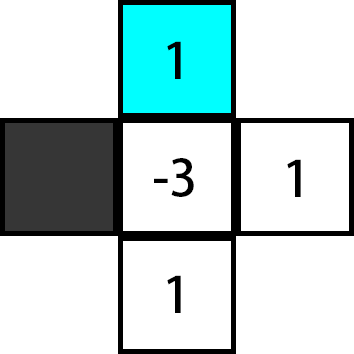
\includegraphics[width=4cm]{Poisson_Stencil}
\centering
\label{fig:PoissonBoundary}
\caption{A finite difference Poisson stencil on the boundary. White cells are interiors cell, i.e. they are degrees of freedom. Blue cell are Dirichlet condition, or essential conditions, that their value are prescribed. Grey cells are exterior cells that are not part of the domain $\Omega$. The face between gray and white cell describes a Nuemann condition, or a nature boundary.}
\end{figure}

But even though we may assume that the boundary conditions are cell aligned at the finest level, this may not holds true for the coarse levels, when the cell size doubles. Figure ~\ref{fig:GeometricCoarsening} demonstrates the heuristic for coarsening boundary conditions. Note that after coarsening, the coarse level discretization may not be of the same order of accuracy to the continuous PDE as the finest level at the boundaries. This inconsistent boundary conditions break the principle that the each level of the multigrid hierarchy should be the discretization of the \textbf{same} continuous PDE. But to compensate this discrepancy, we can introduce additional boundary smoothing to stabilize the multigrid.
\begin{figure}[t]
\centering
\begin{minipage}{.5\textwidth}
  \centering
  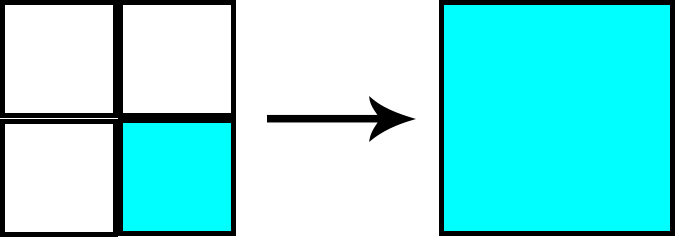
\includegraphics[width=.8\linewidth]{Dirichlet_Coarsening}
\end{minipage}%
\begin{minipage}{.5\textwidth}
  \centering
  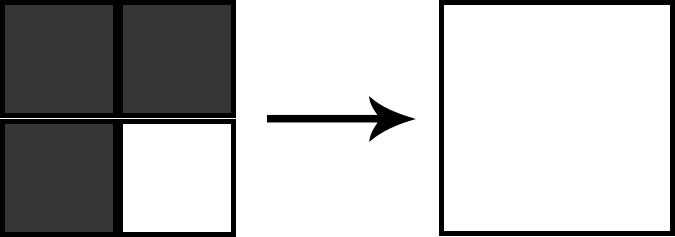
\includegraphics[width=.8\linewidth]{Nuemann_Coarsening}
\end{minipage}
  \caption{Geometric coarsening of the simulation domain. Left: if one of the cells is Dirichlet cell, we will coarsen it as Dirichlet cell at the coarse level, Right: otherwise if one of the cells is interior cell, we will coarsen it as interior cell at the coarse level}
  \label{fig:GeometricCoarsening}
\end{figure}
